\documentclass[12pt,twoside]{scrartcl}
\usepackage[a4paper,top=2cm,left=2cm,right=2cm,bottom=2cm,includefoot,includehead]{geometry}
\usepackage{graphicx}
\usepackage[numbers]{natbib} % Add this line for natbib package
\usepackage{fancyhdr}
\usepackage{hyperref}
\usepackage{amsmath}
\usepackage{circuitikz}
\graphicspath{ {figures/} }


\ctikzset{
    resistor = american,
    % inductor = american,
    voltage = raised ,
    voltage dir = old,
    quadpoles/transformer core/inner = 1, %Eliminates the horizontal bars on the transformer
    quadpoles/transformer core/width = 0.8, %Adjusts the width so that the transformers are closer
    diodes/scale = 0.6,
    capacitors/scale = 0.6,
    resistors/scale = 0.6,
    inductors/scale = 0.8,
    % bipoles/label_distance = 4pt,
    % switch/scale = 0.8,
    % bipoles/length = 1cm,
}

%% shifted open voltage 
\tikzset{open shifted/.style={
    open ,open voltage position=legacy, voltage shift=-0.9}
}

\pagestyle{fancy} % Set the page style to fancy
\fancyhf{} % Clear all header and footer fields

% Define the header and footer content for odd and even pages
\fancyhead[CE]{School of Electrical and Computer Engineering}
\fancyhead[CO]{Power Electronics and Renewable Energy Systems} % Left header on even pages, right header on odd pages
% \fancyhead[RE,LO]{Right Header} % Right header on even pages, left header on odd pages
\fancyfoot[LE,RO]{\thepage} % Page number on left footer of even pages and right footer of odd pages
% \fancyfoot[RE,LO]{ELEC3251} % Left footer on odd pages, right footer on even pages

\begin{document}
\pagenumbering{arabic}
\setcounter{page}{1}
\begin{titlepage}
    \begin{center}

        
\includegraphics[width=0.2\textwidth]{LOGO_Square.pdf}

        \vspace*{0.4cm}
        School of Electrical and Computer Engineering \\
        University of Newcastle, Australia
        
        \vspace{1cm}
        \huge
        \textbf{\textsf{ELEC3251 \\ }}
        \vspace{0.2cm}
        \huge
        \textbf{\textsf{Assignment 2}}

        \vspace{0.5cm}
        \large
        \textbf{\textsf{Analysis of Switching Harmonics, \\ 
                        Grid Connected Inverters and \\ 
                        Space Vector Control System Design
                        }}

        \vspace{1.5cm}
        \normalsize
        Liam Patey-Dennis \\
        c3349900
        \vfill    
    \end{center}
\end{titlepage}


\section{PV Voltage and Switching Harmonics}
\subsection{Method}
To determine the correct switching output, a test was performed at the H-bridge output to confirm that both
switching strategies can be achieved. 
This test involved setting a constant sinusoid input at the H-bridge controller.
\begin{figure}[htp]
    \centering
    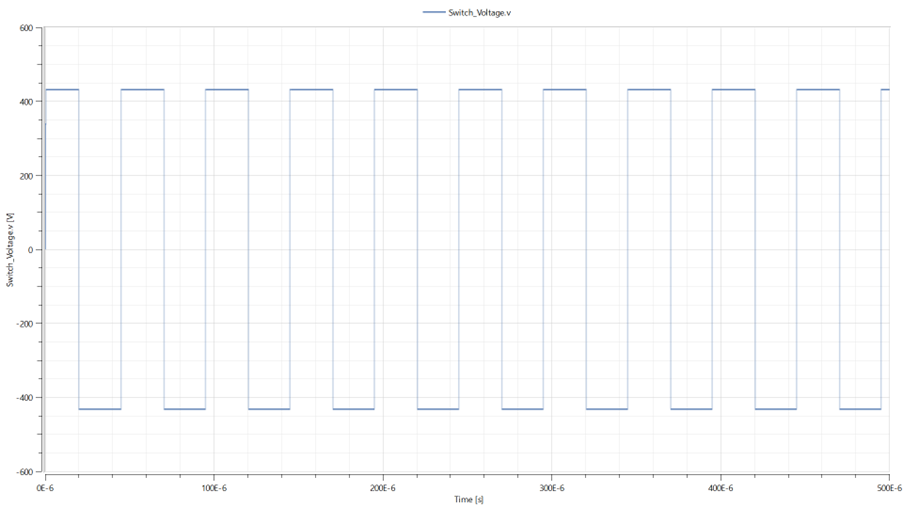
\includegraphics[width=0.7\textwidth]{Bipolar_sw.png}
    \caption{Bipolar Switching Test}
    \label{fig:Bipolar Switching}
\end{figure}
\begin{figure}[htp]
    \centering
    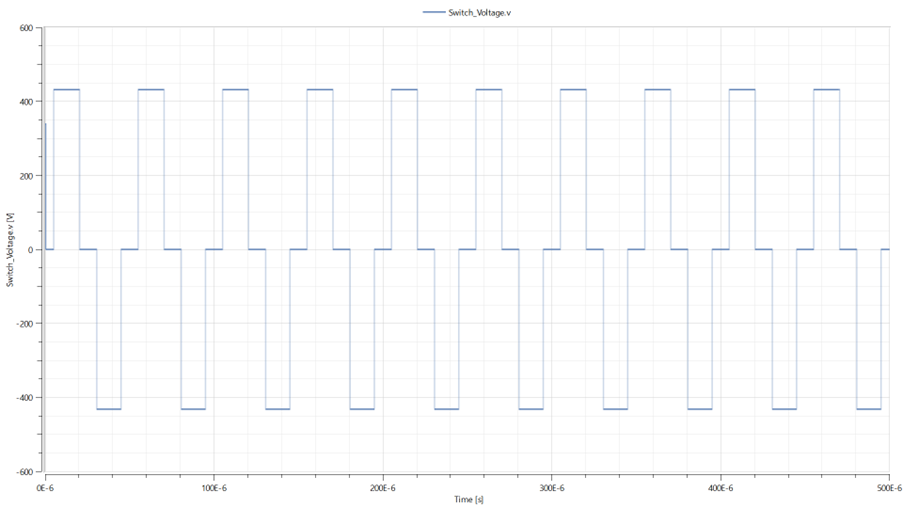
\includegraphics[width=0.7\textwidth]{Unipolar_sw.png}
    \caption{Unipolar Switching Test}
    \label{fig:Unipolar Switching}
\end{figure}
\newpage
\noindent
The switching frequency was set to 20$\: kHz$. The current sensor, Ic was added to measure current 
through the capacitor. The voltage sensor for the capacitor was named Vc. The simulation was run twice, at 0.2 s and at 10 s. This allows the 
viewing of different frequency components. The numbers of cells in series for the solar cell was 850. The capacitance was set to 56 mF. The some experimentation,
it was found that the input supply was 5kW.
\subsection{Results}

\begin{figure}[htp]
    \centering
    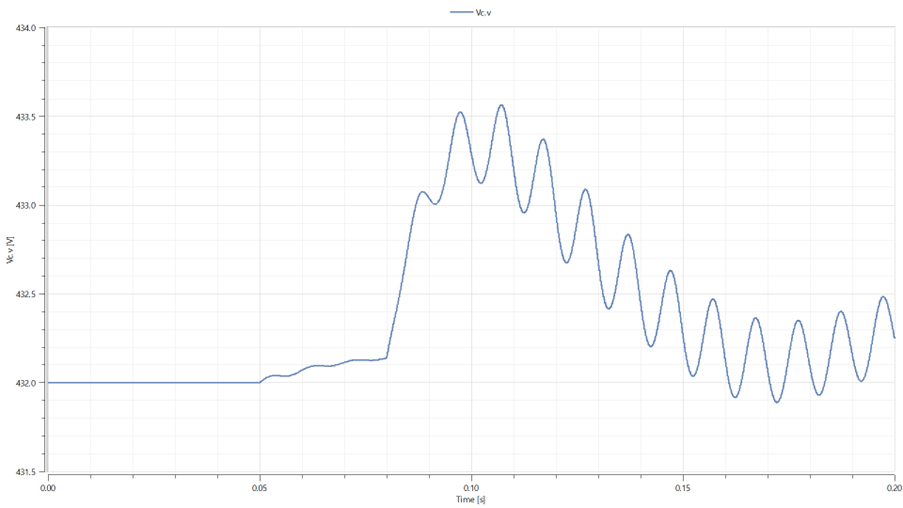
\includegraphics[width=0.75\textwidth]{Bipolar_Vc_0.2.png}
    \caption{Bipolar $V_c$, capacitor voltage (PV to GND), Sim Time = 0.2 s}
    \label{fig:BipolarVc0.2}
\end{figure}
\begin{figure}[htp]
    \centering
    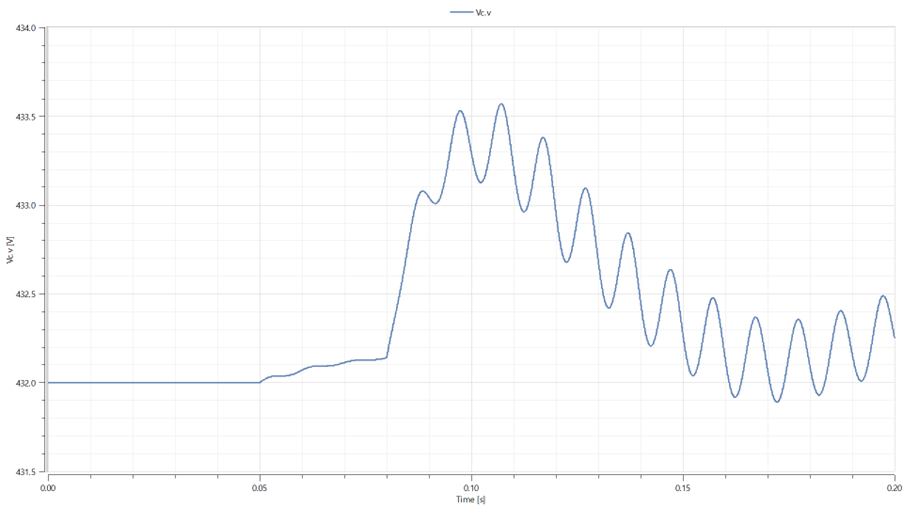
\includegraphics[width=0.75\textwidth]{Unipolar_Vc_0.2.png}
    \caption{Unipolar $V_c$, capacitor voltage (PV to GND), Sim Time = 0.2 s}
    \label{fig:UnipolarVc0.2}
\end{figure}
\begin{figure}[htp]
    \centering
    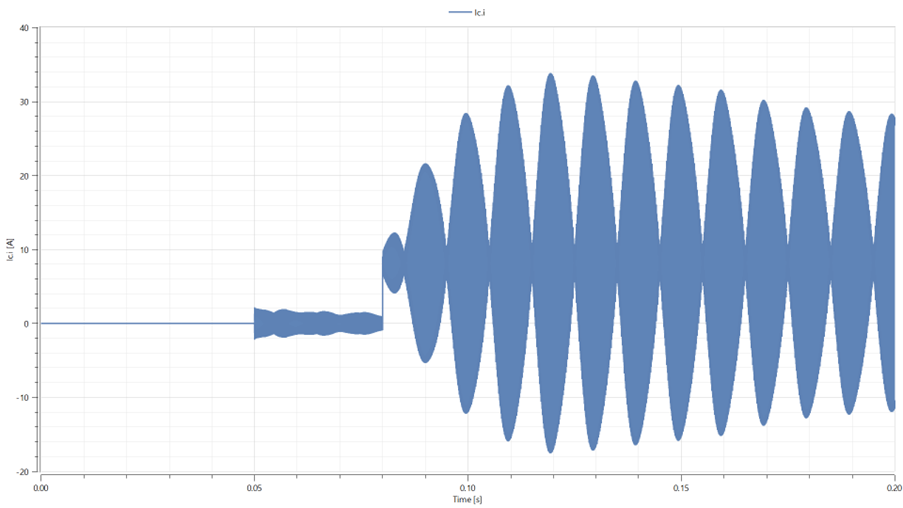
\includegraphics[width=0.8\textwidth]{Bipolar_Ic_0.2.png}
    \caption{Bipolar $I_c$, current through capacitor, Sim Time = 0.2 s}
    \label{fig:BipolarIc0.2}
\end{figure}
\begin{figure}[htp]
    \centering
    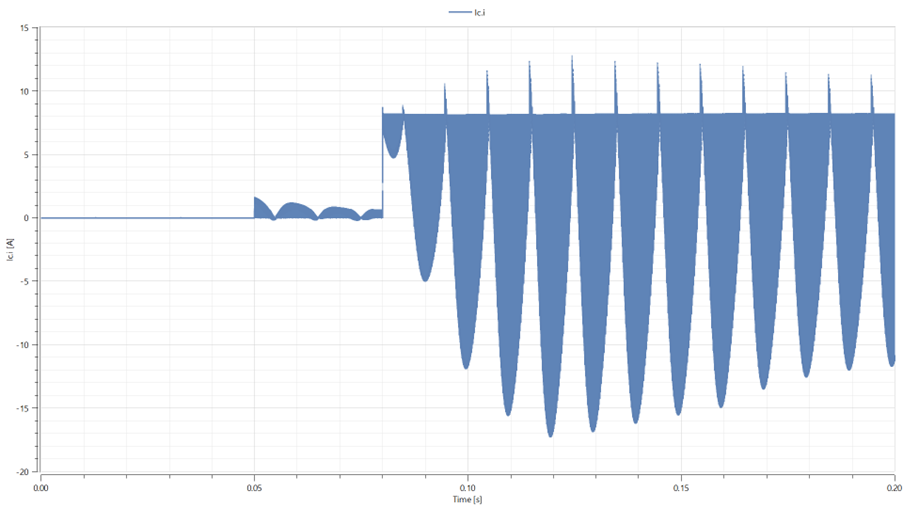
\includegraphics[width=0.8\textwidth]{Unipolar_Ic_0.2.png}
    \caption{Unipolar $I_c$, current through capacitor, Sim Time = 0.2 s}
    \label{fig:UnipolarIc0.2}
\end{figure}
\subsection{Discussion}
In both switching methods, the capacitor voltage (PV) were equal, see Figure 4 \& 5 at \ref{fig:BipolarVc0.2}. 
At time 0.05 s the H-bridge starts switching to produce a current. There are noticable harmonics. This frequency component can 
calculated by measuring its period, which inferred from Figure \ref{fig:BipolarVc0.2} is about 0.01 s. For wave relationship,
\begin{equation}
    f = \dfrac{1}{T}
\end{equation}
Therefore the frequency, $f$, is 100 $Hz$. This comes 
from the grid connected voltage. This is 50 $Hz$,
that makes this signal, the second harmonic. The same frequency can 
be seen from the current plots, Figure \ref{fig:BipolarIc0.2}.
There is a distinct difference between the plots, due to the differnet switching modes, 
see Figure \ref{fig:UnipolarIc0.2}. This is expected, as 
harmonic disturbance should be less under unipolar switching. The greatest piece of 
evidence, can be inferred from the magnitudes of the current plots. 
As the magnitude of the harmonics is from 40 to -20
for bipolar and from 15 to -20 for unpolar. 


\section{Grid Connected Inverters}
\section{Space Vector Control System Design}



\newpage
\bibliographystyle{IEEEtranN}
\bibliography{references}

\end{document}
